\documentclass[14pt, openany, titlepage]{report} % Explicitly use openany and titlepage
\usepackage[utf8]{inputenc}
\usepackage[italian,english]{babel}
\usepackage{graphicx}
\usepackage{cite}
\usepackage{amsmath}
\usepackage[table,xcdraw]{xcolor}
\usepackage[italian]{minitoc}
\usepackage{fancybox}
\usepackage{fancyhdr}
\usepackage{verbatim}
\usepackage{url}
\usepackage{color}
\usepackage{listings}
\usepackage{makeidx}
\usepackage{comment}
\usepackage{hyperref}
\usepackage{bm}
\usepackage{longtable}
\usepackage{tabularx}
\usepackage{placeins}
\usepackage{caption}
\usepackage{float}
\usepackage{xcolor}
\usepackage{soul}
\usepackage{array}
\usepackage{multirow}
\usepackage{adjustbox} % Pacchetto per ridimensionare automaticamente
\usepackage{graphicx} % Per il ridimensionamento
\usepackage{lscape}
\usepackage{mathtools}
\usepackage{amsmath}
\usepackage{amssymb}
\usepackage{listings}
\usepackage[svgnames]{xcolor}
\usepackage{booktabs}

% Set link colors without borders
\hypersetup{
    colorlinks=true,
    linkcolor=black,
    filecolor=magenta,      
    urlcolor=cyan,
}

\lstset{frame=tb,
    language=Java,
    numbers=left,
    keywordstyle=\color{blue},
    alsoletter={.}
}

\lstset{language=R,
    basicstyle=\small\ttfamily,
    stringstyle=\color{DarkGreen},
    otherkeywords={0,1,2,3,4,5,6,7,8,9},
    morekeywords={TRUE,FALSE},
    deletekeywords={data,frame,length,as,character},
    keywordstyle=\color{blue},
    commentstyle=\color{DarkGreen},
}

\graphicspath{ {./Figure/} }


% Minimize additional blank pages
\let\cleardoublepage\clearpage % Suppresses new page on odd side
\flushbottom % Avoid vertical blank space between paragraphs

% Title Page
\begin{document}
\selectlanguage{italian}

\begin{titlepage}
\begin{center}
    \begin{figure}
        
\includegraphics[width=3.5cm, height=3.5cm]{unisa.png}
        \centering
    \end{figure}
    {\Large Università degli Studi di Salerno}\\[0.2truecm]
    {\large Dipartimento di Informatica\\Corso di Laurea Triennale in Informatica}\\
    \hrulefill
    \vfill
    {\large Progetto Calcolo Probabilità Statistica Matematica\\(CPSM)}\\[0.1truecm]
    \vfill\vfill
    {\LARGE {\bf Indagine Statistica sulle\\[0.1truecm]Morti in incidenti stradali}}
    \vfill\vfill
    
    \hfill  \textbf{Tozza Gennaro Carmine}
    \centerline{\hfill Matricola: 0512120382}
    
    \vfill
    \hrulefill 
    \begin{center} Anno Accademico 2024-2025 \end{center}
\end{center}
\end{titlepage}

% Suppress page break after table of contents
\tableofcontents

\chapter{Introduzione}
\section{Problematica}
Gli \textbf{incidenti stradali} costituiscono una delle principali emergenze 
di sanità pubblica, in quanto responsabili ogni anno di un elevato 
numero di decessi, in particolare tra i giovani, e di gravi conseguenze
 in termini di disabilità temporanee e permanenti, oltre al drammatico impatto umano e psicologico sulle vittime e 
 sulle loro famiglie. 
\noindent

\section{Scopo del progetto}
Il progetto consiste nel realizzare un’indagine statistica \footnote{\url{https://siqual.istat.it/SIQual/visualizza.do?id=7777778&refresh=true&language=IT}}sugli incidenti stradali verificatisi sulla rete stradale del territorio nazionale, tra il 2010 e il 2023 verbalizzati da un'autorità di Polizia o dai Carabinieri, 
avvenuti su una strada aperta alla circolazione pubblica e che hanno causato morti (entro il 30° giorno) con il coinvolgimento 
di almeno un veicolo. \\\\
\noindent
La rilevazione è condotta correntemente dall’Istat, con la compartecipazione dell'ACI e di numerosi Enti pubblici istituzionali, 
è a carattere totale e a cadenza mensile (inserita tra le rilevazioni di interesse pubblico nel Programma Statistico Nazionale - PSN - IST00142). \\\\
\noindent
Per l'analisi dei dati è stato scelto l'ambiente di calcolo statistico \textbf{R}. \\
R fornisce un'ampia varietà di tecniche statistiche (modellazione lineare e non lineare, test statistici classici, analisi delle serie temporali, classificazione, \dots)
e grafiche ed è altamente estensibile.\\\\
\noindent
Uno dei punti di forza di R è la facilità con cui possono essere prodotti grafici ben progettati e di qualità per la pubblicazione, 
compresi simboli matematici e formule se necessario.\\\\
\noindent
Per semplificare l'analisi, si è scelto di lavorare non sull'intero dataset, 
ma su un sottoinsieme filtrato di dati, relativo alle \textbf{morti per incidenti stradali che riguardano solo i conducenti di età compresa tra i 21 e i 24 anni.}\\\\
\noindent
Per approfondire l'analisi con dati dettagliati e specifici, è possibile consultare il dataset direttamente sul sito dell'ISTAT al seguente link:
\url{https://esploradati.istat.it/databrowser/#/it/dw/categories/IT1,Z0810HEA,1.0/HEA_ROAD/IT1,41_270_DF_DCIS_MORTIFERITISTR1_1,1.0}\\\\
\noindent
Il dataset in formato \textbf{CSV(Comma-Separated Values)} è stato ottenuto dalla fonte ISTAT tramite il link indicato, assicurando così l'affidabilità dei dati.\\\\
Il formato scelto (CSV) permette un'agevole manipolazione dei dati, essendo compatibile con la maggior parte dei software statistici e
dei fogli di calcolo, ottimizzando l'analisi e la visualizzazione delle informazioni.\\

\begin{table}[!ht]
\centering
\footnotesize
\begin{tabularx}{\textwidth}{|l|*{14}{>{\centering\arraybackslash}X|}}
\hline
\textbf{Intersezione} & \textbf{'10} & \textbf{'11} & \textbf{'12} & \textbf{'13} & \textbf{'14} & \textbf{'15} & \textbf{'16} & \textbf{'17} & \textbf{'18} & \textbf{'19} & \textbf{'20} & \textbf{'21} & \textbf{'22} & \textbf{'23} \\ 
\hline
Incrocio & 55 & 45 & 42 & 23 & 34 & 24 & 28 & 25 & 23 & 13 & 15 & 16 & 21 & 10 \\ \hline
Rotatoria & 7 & 4 & 2 & 5 & 5 & 1 & 5 & 3 & 1 & 2 & 1 & 2 & -- & 3 \\ \hline
Rettilineo & 92 & 102 & 89 & 82 & 96 & 95 & 66 & 70 & 60 & 72 & 66 & 69 & 69 & 74 \\ \hline
Curva & 58 & 51 & 48 & 46 & 45 & 44 & 41 & 36 & 38 & 42 & 23 & 40 & 27 & 38 \\ \hline
Dosso/Pend. & 2 & 7 & 2 & 4 & 2 & 3 & 5 & 1 & 2 & 3 & 2 & 4 & 3 & 1 \\ \hline
Galleria & 1 & 1 & 1 & 1 & -- & 1 & 1 & 1 & -- & -- & 3 & 1 & -- & -- \\ \hline
\hline
\textbf{Totale} & 215 & 210 & 184 & 161 & 182 & 168 & 146 & 136 & 124 & 132 & 110 & 132 & 120 & 126 \\ \hline
\end{tabularx}
\end{table}

\normalsize


\chapter{Tabelle delle frequenze}

\begin{center}
\begin{lstlisting}[breaklines=true]
# inclusione librerie
library("tidyverse")
require("tidyverse")
library("dplyr")

# viene caricato il dataset
dati <- read.csv("dati_istat.csv")

# filtraggio dati
dati <- dati %>% select(Intersezione, TIME_PERIOD, Osservazione) 
dati <- dati %>% 
  filter(Intersezione != "Totale") 

# 1. Frequenze assolute per intersezione dell'incidente
freq_assolute <- aggregate(Osservazione ~ Intersezione, data=dati, sum)
colnames(freq_assolute) <- c("Intersezione", "Frequenza_Assoluta")
print(freq_assolute)

# 2. Frequenze relative per intersezione dell'incidente
totale <- sum(freq_assolute$Frequenza_Assoluta)
freq_assolute$Frequenza_Relativa <- freq_assolute$Frequenza_Assoluta / totale
print(freq_assolute)

# 3. Frequenze cumulate assolute
freq_assolute <- freq_assolute[order(-freq_assolute$Frequenza_Assoluta),]
freq_assolute$Frequenza_Cumulata_Assoluta <- cumsum(freq_assolute$Frequenza_Assoluta)
print(freq_assolute)

# 4. Frequenze cumulate relative
freq_assolute$Frequenza_Cumulata_Relativa <- freq_assolute$Frequenza_Cumulata_Assoluta / totale
print(freq_assolute)
\end{lstlisting}  
\end{center}

\noindent
L'output generato dal codice R riportato è sintetizzato
 nella seguente tabella:

\begin{table}[!ht]
\centering
\footnotesize
\begin{tabularx}{\textwidth}{|l|>{\centering\arraybackslash}X|>{\centering\arraybackslash}X|>{\centering\arraybackslash}X|>{\centering\arraybackslash}X|}
\hline
\textbf{Tipo intersezione} & \textbf{Freq. Assoluta} & \textbf{Freq. Relativa} & \textbf{Freq. Cum. Assoluta} & \textbf{Freq. Cum. Relativa} \\ 
\hline
Rettilineo & 1102 & 0.5135 & 1102 & 0.5135 \\ \hline
Curva & 577 & 0.2689 & 1679 & 0.7824 \\ \hline
Incrocio & 374 & 0.1743 & 2053 & 0.9567 \\ \hline
Dosso/Pendenza/Strettoia & 41 & 0.0191 & 2094 & 0.9758 \\ \hline
Rotatoria & 41 & 0.0191 & 2135 & 0.9949 \\ \hline
Galleria & 11 & 0.0051 & 2146 & 1.0000 \\ \hline
\end{tabularx}
\end{table}
\normalsize

\chapter{Rappresentazione dei dati mediante grafici}
\begin{center}
\begin{lstlisting}[breaklines=true]
# 1. Grafico frequenza assolute
barplot(freq_assolute$Frequenza_Assoluta, 
        names.arg = freq_assolute$Intersezione,
        main = "Frequenze assolute per intersezione",
        xlab = "",
        ylab = "",
        col = "steelblue",
        las = 2) # Etichette verticali
\end{lstlisting}  
\end{center}

\begin{figure}[H] % H forza la posizione esatta
    \centering
    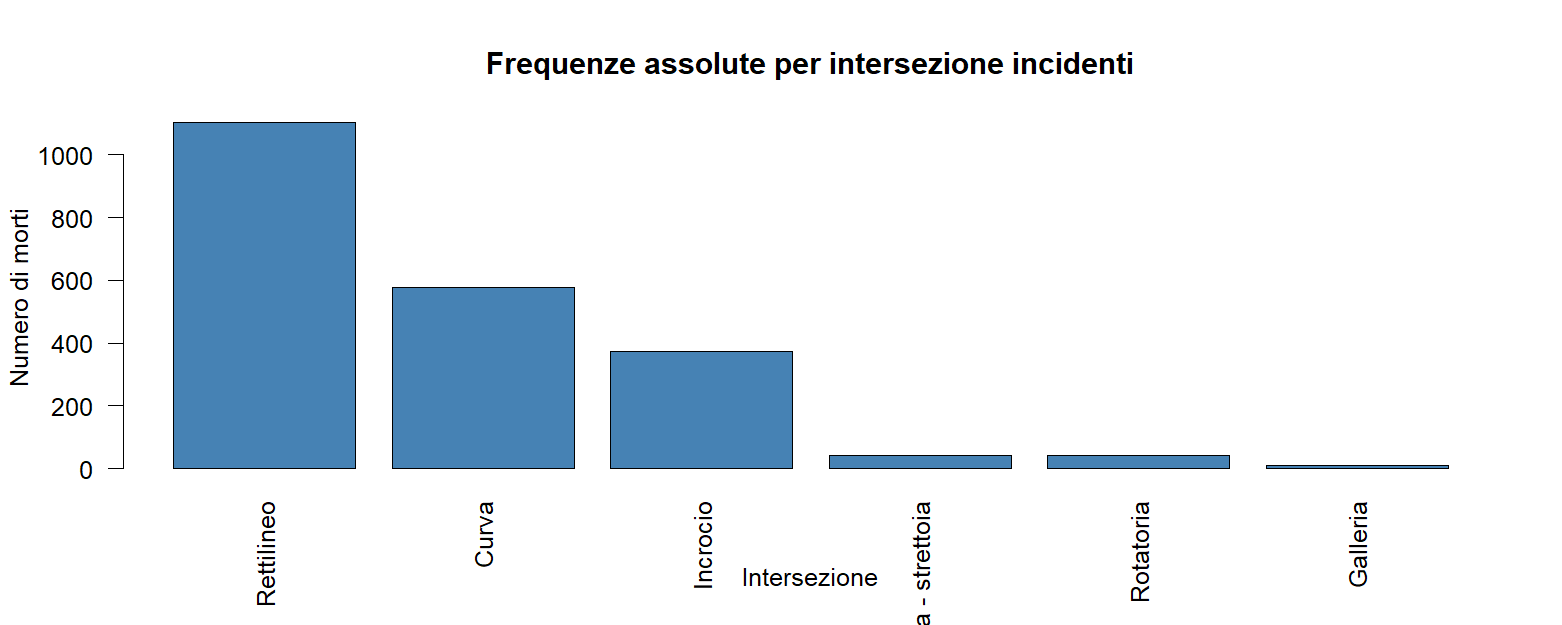
\includegraphics[width=12cm, height=7cm]{Rplot.png} % Adatta l'immagine alla larghezza del testo
\end{figure}

\begin{center}
\begin{lstlisting}[breaklines=true]
# 2. Grafico frequenze relative
barplot(freq_assolute$Frequenza_Relativa, 
        names.arg = freq_assolute$Intersezione,
        main = "Frequenze Relative per Intersezione",
        xlab = "",
        ylab = "",
        col = "coral",
        las = 2,
        cex.names = 0.8)
\end{lstlisting}  
\end{center}

\begin{figure}[H] % H forza la posizione esatta
    \centering
    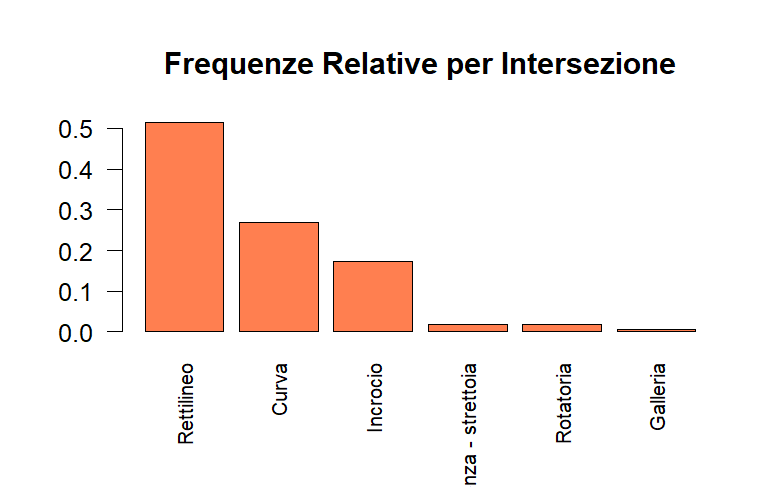
\includegraphics[width=12cm, height=7cm]{Rplot03.png} % Adatta l'immagine alla larghezza del testo
\end{figure}

\begin{center}
\begin{lstlisting}[breaklines=true]
# 3. Grafico frequenze cumulate assolute
barplot(freq_assolute$Frequenza_Cumulata_Assoluta, 
        names.arg = freq_assolute$Intersezione,
        main = "Frequenze Cumulate Assolute",
        xlab = "",
        ylab = "",
        col = "darkgreen",
        las = 2,
        cex.names = 0.8)
\end{lstlisting}  
\end{center}

\begin{figure}[H] % H forza la posizione esatta
    \centering
    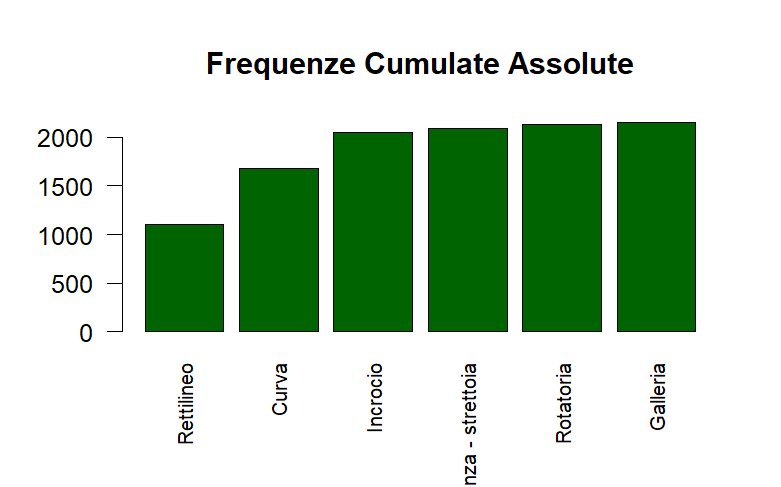
\includegraphics[width=12cm, height=7cm]{Rplot04.png} % Adatta l'immagine alla larghezza del testo
\end{figure}

\begin{center}
\begin{lstlisting}[breaklines=true]
# 4. Grafico frequenze cumulate relative
barplot(freq_assolute$Frequenza_Cumulata_Relativa, 
        names.arg = freq_assolute$Intersezione,
        main = "Frequenze Cumulate Relative",
        xlab = "",
        ylab = "",
        col = "purple",
        las = 2,
        cex.names = 0.8)
\end{lstlisting}  
\end{center}

\begin{figure}[H] % H forza la posizione esatta
    \centering
    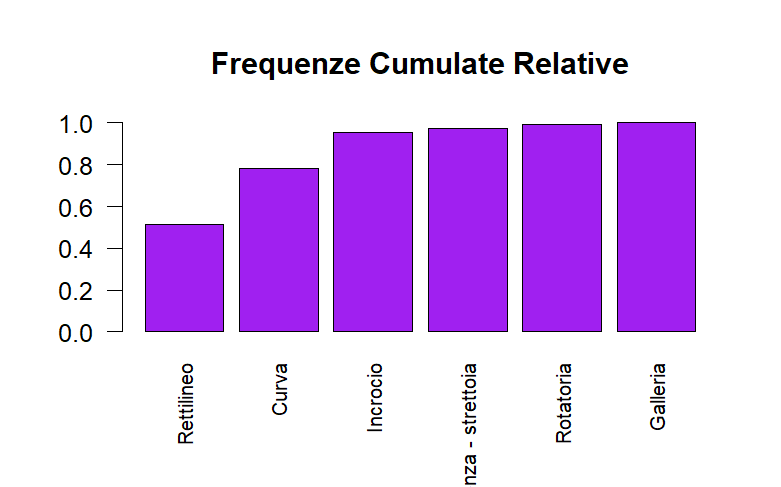
\includegraphics[width=12cm, height=7cm]{Rplot05.png} % Adatta l'immagine alla larghezza del testo
\end{figure}


\begin{center}
\begin{lstlisting}[breaklines=true]
# Converti TIME_PERIOD in fattore per mantenere l'ordine originale
dati$TIME_PERIOD <- factor(dati$TIME_PERIOD, levels = unique(dati$TIME_PERIOD))

# Calcola il numero totale di morti per anno
morti_per_anno <- dati %>%
  group_by(TIME_PERIOD) %>%
  summarise(Totale_Morti = sum(Osservazione, na.rm = TRUE))

# Crea il grafico a linee con tutti gli anni visibili
ggplot(morti_per_anno, aes(x = TIME_PERIOD, y = Totale_Morti, group = 1)) +
  geom_line(color = "steelblue", size = 1) +
  geom_point(color = "steelblue", size = 2) +
  labs(title = "Andamento del numero di morti per incidenti stradali",
       x = "Anno",
       y = "Numero di morti") +
  theme_minimal() +
  theme(plot.title = element_text(hjust = 0.5),
        axis.text.x = element_text(angle = 45, hjust = 1, size = 8)) +  # Riduci dimensione testo
  scale_x_discrete(breaks = levels(morti_per_anno$TIME_PERIOD))  # Mostra tutti i valori
\end{lstlisting}  
\end{center}

\begin{figure}[H] % H forza la posizione esatta
    \centering
    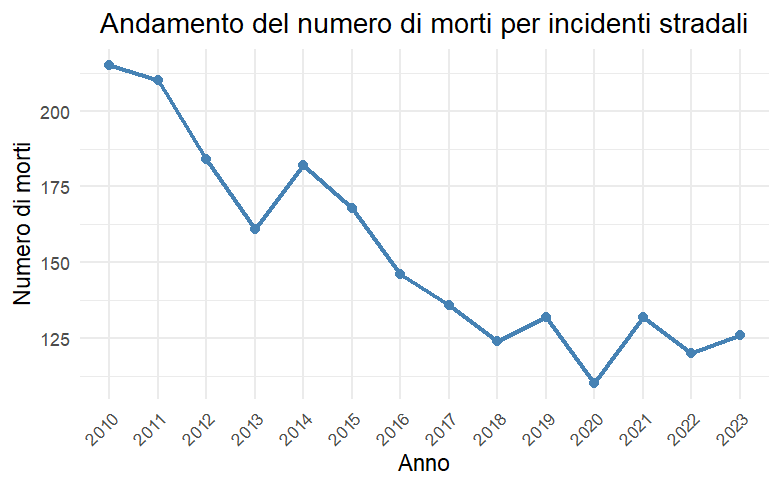
\includegraphics[width=12cm, height=7cm]{Rplot01.png} % Adatta l'immagine alla larghezza del testo
\end{figure}

\newpage

\begin{center}
\begin{lstlisting}[breaklines=true]
# Crea il grafico a torta
ggplot(freq_assolute, aes(x = "", y = Frequenza_Assoluta, fill = Intersezione)) +
  geom_bar(width = 1, stat = "identity") +
  coord_polar("y", start = 0) +
  labs(title = "",
       fill = "Tipo di intersezione") +
  theme_void() +
  theme(plot.title = element_text(hjust = 0.5, size = 14, face = "bold"),
        legend.position = "right") +
  geom_text(aes(label = paste0(round(Frequenza_Assoluta/sum(Frequenza_Assoluta)*100, 1), "%")), 
            position = position_stack(vjust = 0.5),
            size = 3)
\end{lstlisting}  
\end{center}

\begin{figure}[H] % H forza la posizione esatta
    \centering
    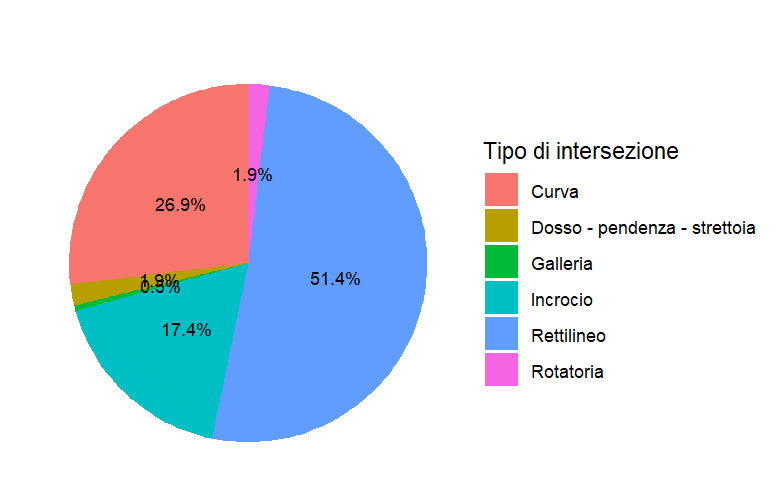
\includegraphics[width=13cm, height=8cm]{Rplot08.png} % Adatta l'immagine alla larghezza del testo
\end{figure}



\chapter{Indici di posizione}
In questo capitolo verranno calcolati gli \textbf{indici di posizione} 
sulla variabile numerica \texttt{Osservazione} del dataset 
\texttt{dati}. \\\\
\noindent
Questa variabile rappresenta il numero di morti
 registrato per una specifica combinazione di tipo di intersezione 
 e anno, limitatamente alla fascia di età dei conducenti tra 21 e 24 
 anni. \\\\
 \noindent
 Gli indici di posizione(o di tendenza generale) sono misure che consentono di 
 sintetizzare i dati osservati con un solo valore numerico che sia rappresentativo dei dati stessi.
 Gli indici di posizone più adoperati sono tre
\begin{itemize}
  \item media
  \item mediana
  \item moda
\end{itemize}

\section{Media campionaria}
La \textbf{media campionaria} è la somma di tutte le osservazioni divisa per il numero di osservazioni.
 Fornisce una misura del valore centrale della distribuzione.
\begin{center}
\begin{lstlisting}[breaklines=true]
media_generale <- mean(dati$Osservazione, na.rm = TRUE)
print(paste("Media campionaria generale delle osservazioni:", round(media_generale, 2)))
\end{lstlisting}  
\end{center}
\noindent
Output: 
\begin{verbatim}
"Media campionaria generale delle osservazioni: 27.51"
\end{verbatim}
Questo valore indica che, in media, per ogni specifica combinazione di tipo di intersezione e anno considerata nel dataset filtrato, si sono registrati circa 27.51 decessi.

\section{Mediana campionaria}
La \textbf{mediana} è un numero che precede tanti dati quanti ne segue, ossia il 
valore centrale dei dati riordinati in senso crescente.
\begin{center}
\begin{lstlisting}[breaklines=true]
mediana_generale <- median(dati$Osservazione, na.rm = TRUE)
print(paste("Mediana generale delle osservazioni:", mediana_generale))
\end{lstlisting}  
\end{center}
\noindent
Output:
\begin{verbatim}
"Mediana generale delle osservazioni: 15.5"
\end{verbatim}
 Il fatto che la mediana (15.5)
 sia inferiore alla media (27.51) suggerisce una distribuzione 
 asimmetrica a destra.

\section{Moda campionaria}
La \textbf{moda} è il valore (o i valori, in caso di distribuzioni multimodali)
 che appare più frequentemente in un insieme di dati.
\begin{center}
\begin{lstlisting}[breaklines=true]
find_mode <- function(x) {
    u <- unique(x)
    tab <- tabulate(match(x, u))
    u[tab == max(tab)]
  }

find_mode(dati$Osservazione)
\end{lstlisting}  
\end{center}
\noindent
Output:
\begin{verbatim}
  1 
\end{verbatim}
L'output '1', indica che il numero di decessi 
più frequentemente osservato per una singola combinazione 
intersezione/anno è 1. Se ci fossero più valori con la stessa 
frequenza massima, sarebbero elencati tutti.


\chapter{Indici di variabilità} 
Di seguito calcoliamo gli \textbf{indici di variabilità(o di dispersione)}, che descrivono la 
variabilità dei dati osservati e consentono di valutare l'informazione 
fornita dall'indice di posizione utilizzato, dando dei dati più accurati.

\section{Varianza campionaria}
La \textbf{varianza campionaria ($s^2$)} misura la dispersione
media quadratica dei dati attorno alla media campionaria.
È espressa nell'unità di misura dei dati al quadrato.
\begin{center}
\begin{lstlisting}[breaklines=true]
# Calcolo della varianza sulla variabile 'Osservazione'.
varianza_campionaria <- var(dati$Osservazione, na.rm = TRUE)
print(paste("Varianza campionaria delle osservazioni:", round(varianza_campionaria, 2)))
\end{lstlisting}
\end{center}
\noindent
Output (valore basato sulla media e mediana fornite, è una stima):
\begin{verbatim}
"Varianza campionaria delle osservazioni: 859.52" 
\end{verbatim}
Un valore elevato della varianza indica una notevole
 dispersione dei dati attorno alla media.
    
\section{Deviazione standard campionaria}
La \textbf{deviazione standard campionaria ($s$)} è la radice quadrata 
della varianza campionaria. Fornisce una misura della dispersione
 media dei dati attorno alla media, espressa nella stessa unità 
 di misura dei dati originali, rendendola più interpretabile 
 della varianza.
\begin{center}
\begin{lstlisting}[breaklines=true]
# Calcolo della deviazione standard sulla variabile 'Osservazione'.
dev_std_campionaria <- sd(dati$Osservazione, na.rm = TRUE)
print(paste("Deviazione standard campionaria delle osservazioni:", round(dev_std_campionaria, 2)))
\end{lstlisting}
\end{center}
\noindent
Output (radice quadrata della varianza stimata):
\begin{verbatim}
"Deviazione standard campionaria delle osservazioni: 29.61"
\end{verbatim}
Questo valore indica che, mediamente, i singoli conteggi di 
decessi si discostano dalla media campionaria (27.51) di 
circa 29.61 unità.
    
\section{Scarto medio assoluto}
Lo \textbf{scarto medio assoluto (Mean Absolute Deviation, MAD)}
 dalla media è la media delle deviazioni assolute (cioè, senza segno)
  dei dati dalla loro media. Come la deviazione standard, 
  misura la dispersione media, ma è meno sensibile ai valori 
  anomali perché non eleva al quadrato gli scarti.
\begin{center}
\begin{lstlisting}[breaklines=true]
# Calcolo dello scarto medio assoluto dalla media per 'Osservazione'.
media_oss <- mean(dati$Osservazione, na.rm = TRUE)
scarto_medio_assoluto <- mean(abs(dati$Osservazione - media_oss), na.rm = TRUE)
print(paste("Scarto medio assoluto (dalla media) delle osservazioni:", round(scarto_medio_assoluto, 2)))
\end{lstlisting}
\end{center}
\noindent
Output (stima):
\begin{verbatim}
"Scarto medio assoluto (dalla media) delle osservazioni: 25.13"
\end{verbatim}
In media, le osservazioni si discostano (in valore assoluto) 
dalla media di circa 25.13 decessi.

\section{Ampiezza del campo di variazione}
L'\textbf{ampiezza del campo di variazione (o semplicemente "range")} 
è la differenza tra il valore massimo e il valore minimo osservato 
nel dataset. È una misura di variabilità semplice ma molto sensibile 
ai valori estremi.
\newpage
\begin{center}
\begin{lstlisting}[breaklines=true]
# Calcolo del minimo, massimo e ampiezza del campo di variazione per 'Osservazione'.
min_oss <- min(dati$Osservazione, na.rm = TRUE)
max_oss <- max(dati$Osservazione, na.rm = TRUE)
ampiezza_variazione <- max_oss - min_oss 

print(paste("Valore minimo delle osservazioni:", min_oss))
print(paste("Valore massimo delle osservazioni:", max_oss))
print(paste("Ampiezza del campo di variazione delle osservazioni:", ampiezza_variazione))
\end{lstlisting}
\end{center}
\noindent
Output:
\begin{verbatim}
"Valore minimo delle osservazioni: 1" 
"Valore massimo delle osservazioni: 102" 
"Ampiezza del campo di variazione delle osservazioni: 101"
\end{verbatim}


\section{Coefficiente di variazione}
Il \textbf{coefficiente di variazione (CV)} è una misura di variabilità relativa,
 data dal rapporto tra la deviazione standard e la media (in valore assoluto).
\begin{center}
\begin{lstlisting}[breaklines=true]
# Calcolo del coefficiente di variazione per 'Osservazione'.
media_oss <- mean(dati$Osservazione, na.rm = TRUE)
dev_std_oss <- sd(dati$Osservazione, na.rm = TRUE)
coeff_variazione <- (dev_std_oss / abs(media_oss)) * 100 # abs() per media se potesse essere negativa
print(paste("Coefficiente di variazione delle osservazioni:", round(coeff_variazione, 2), "%"))
\end{lstlisting}
\end{center}
\noindent
Output(in percentuale):
\begin{verbatim}
"Coefficiente di variazione delle osservazioni: 107.6 %"
\end{verbatim}
Un CV del 107.6\% indica una variabilità molto elevata rispetto alla 
media. Questo è coerente con il fatto che la deviazione standard (29.61)
 è addirittura leggermente superiore alla media (27.51), suggerendo una
  notevole eterogeneità nei conteggi dei decessi.
\FloatBarrier


\chapter{Indici di forma}
Gli \textbf{indici di forma} misurano caratteristiche relative alla forma della distribuzione
dati. I più usati sono l'indice di asimmetria e l'indice di curtosi.

\section{Indice di asimmetria}
L'\textbf{indice di asimmetria (skewness)} misura il grado di simmetria di
 una distribuzione di dati attorno alla sua media.
\begin{itemize}
    \item Un valore di \textbf{skewness $>$ 0} indica un'asimmetria positiva (coda a destra): la distribuzione ha una coda che si estende maggiormente verso i valori più alti. La media è tipicamente maggiore della mediana.
    \item Un valore di \textbf{skewness $<$ 0} indica un'asimmetria negativa (coda a sinistra): la distribuzione ha una coda che si estende maggiormente verso i valori più bassi. La media è tipicamente minore della mediana.
    \item Un valore di \textbf{skewness $\approx$ 0} indica una distribuzione approssimativamente simmetrica (come la distribuzione normale).
\end{itemize}

\begin{center}
\begin{lstlisting}[breaklines=true]
# Calcolo dell'indice di asimmetria per 'Osservazione'.
indice_asimmetria <- skewness(dati$Osservazione, na.rm = TRUE)
print(paste("Indice di asimmetria (Skewness) delle osservazioni:", round(indice_asimmetria, 2)))
\end{lstlisting}
\end{center}
\noindent
Output:
\begin{verbatim}
"Indice di asimmetria (Skewness) delle osservazioni: 0.9"
\end{verbatim}
Un valore di 0.9 indica una moderata asimmetria positiva
(coda a destra). Questo è coerente con l'osservazione precedente
che la media (27.51) è maggiore della mediana (15.5), suggerendo 
che ci sono alcune osservazioni con un numero di decessi relativamente
alto che "stirano" la coda destra della distribuzione.\\

\noindent
Per visualizzare graficamente questa asimmetria, 
possiamo generare un istogramma con una curva di densità 
sovrapposta e linee verticali per la media e la mediana.

\begin{center}
\begin{lstlisting}[breaklines=true]
# Creazione del grafico
skewness_plot <- ggplot(dati, aes(x = Osservazione)) +
  geom_histogram(aes(y = ..density..), binwidth = 5, fill = "lightblue", color = "black", alpha = 0.7) +
  geom_density(color = "darkblue", linewidth = 1) +
  geom_vline(aes(xintercept = media_oss, color = "Media"), linetype = "dashed", linewidth = 1) +
  geom_vline(aes(xintercept = mediana_generale, color = "Mediana"), linetype = "dotted", linewidth = 1) +
  labs(title = "Distribuzione del Numero di Osservazioni (Decessi)",
       subtitle = paste0("Skewness: ", round(indice_asimmetria, 2), 
                         " | Media: ", round(media_oss, 2), 
                         " | Mediana: ", round(mediana_generale, 2)),
       x = "Numero di Osservazioni (Decessi)",
       y = "Densita") +
  scale_color_manual(name = "Statistiche", values = c("Media" = "red", "Mediana" = "green")) +
  theme_minimal()

print(skewness_plot)
\end{lstlisting}
\end{center}

\begin{figure}[H] 
    \centering
    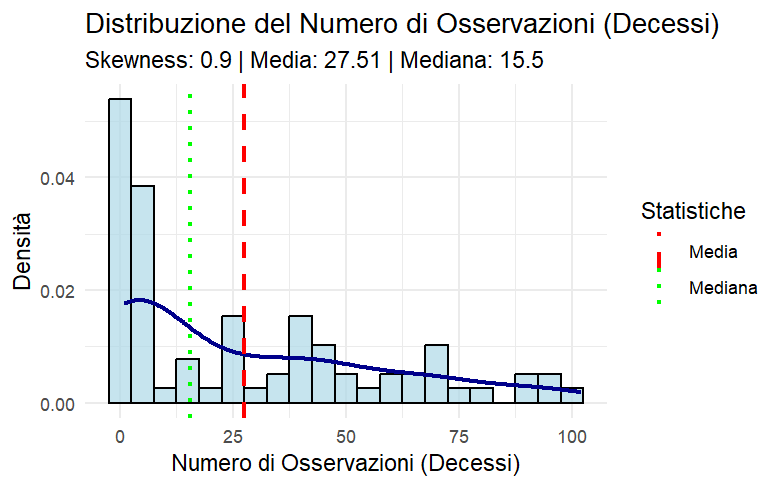
\includegraphics[width=12cm, height=7cm]{Rplot06.png} 
\end{figure}

\section{Indice di curtosi} 
L'\textbf{indice di curtosi} misura l'appiattimento di
 una distribuzione, in particolare la concentrazione dei dati attorno
  al valore centrale e la "pesantezza" delle code, rispetto a una 
  distribuzione normale.
\begin{itemize}
    \item \textbf{Eccesso di curtosi $>$ 0} (Curtosi $>$ 3): Distribuzione leptocurtica. È più appuntita al centro e ha code più pesanti (maggior probabilità di valori estremi) rispetto a una normale.
    \item \textbf{Eccesso di curtosi $<$ 0} (Curtosi $<$ 3): Distribuzione platicurtica. È più piatta al centro e ha code più leggere rispetto a una normale.
    \item \textbf{Eccesso di curtosi $\approx$ 0} (Curtosi $\approx$ 3): Distribuzione normocurtica. Ha una forma simile a quella di una distribuzione normale in termini di appiattimento.
\end{itemize}

\begin{center}
\begin{lstlisting}[breaklines=true]
# Calcolo dell'indice di curtosi (eccesso di curtosi) per 'Osservazione'.
indice_curtosi <- kurtosis(dati$Osservazione, na.rm = TRUE)
print(paste("Indice di curtosi (eccesso di curtosi) delle osservazioni:", round(indice_curtosi, 2)))
# La curtosi "classica" sarebbe approssimativamente: round(indice_curtosi, 2) + 3
\end{lstlisting}
\end{center}
\noindent
Output:
\begin{verbatim}
"Indice di curtosi (eccesso di curtosi) delle osservazioni: 2.64" 
\end{verbatim}
Un eccesso di curtosi di circa 2.64 (corrispondente a una curtosi
 "classica" di circa 2.64 + 3 = 5.64) indica una distribuzione 
 marcatamente \textbf{leptocurtica.}\\\\
 \noindent
  Questo significa che la distribuzione 
 del numero di decessi per combinazione intersezione/anno presenta
  un picco più pronunciato attorno alla moda/mediana e code più 
  "pesanti" rispetto a una distribuzione normale. \\\\
  \noindent
  Ciò implica una 
  maggiore frequenza di valori vicini al centro, ma anche una
   maggiore probabilità di osservare valori estremi (molto alti,
    data l'asimmetria positiva) rispetto a quanto ci si aspetterebbe 
    da una distribuzione normale.\\
\newpage
\noindent
Graficamente si ha
\begin{center}
\begin{lstlisting}[breaklines=true]
# Creazione del grafico per la curtosi
kurtosis_plot <- ggplot(dati, aes(x = Osservazione)) +
  geom_histogram(aes(y = ..density..), binwidth = 5, fill = "lightcoral", color = "black", alpha = 0.7) +
  geom_density(color = "darkred", linewidth = 1) +
  geom_vline(aes(xintercept = media_oss, color = "Media"), linetype = "dashed", linewidth = 1) +
  labs(title = "Distribuzione del Numero di Osservazioni (Decessi)",
       subtitle = paste0("Eccesso di Curtosi: ", round(indice_curtosi, 2),
                         " | Media: ", round(media_oss, 2)),
       x = "Numero di Osservazioni (Decessi)",
       y = "Densita") +
  scale_color_manual(name = "Statistiche", values = c("Media" = "blue")) +
  theme_minimal()

print(kurtosis_plot)
\end{lstlisting}
\end{center}

\begin{figure}[H] 
    \centering
    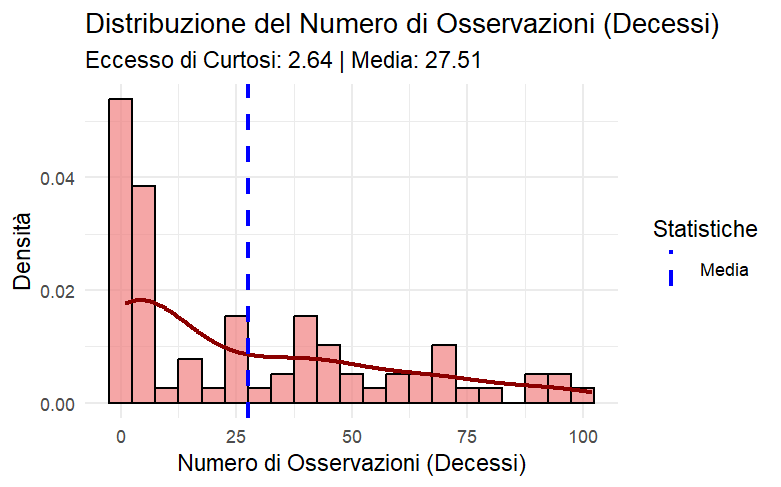
\includegraphics[width=12cm, height=7cm]{Rplot07.png} 
\end{figure}

\chapter{Percentili campionari}
Un \textbf{percentile} k-esimo di un campione di dati è un valore che 
è maggiore di una percentuale k dei dati e minore della 
restante percentuale. \\\\
\noindent
Il 25-esimo percentile si dice primo \textbf{quartile}, il 50-esimo percentile
si dice mediana campionaria o secondo quartile, il 75-esimo percentile
si dice terzo quartile e si denotano con \[Q_{1}, Q_{2}, Q_{3} \].\\
La differenza tra il terzo e il primo quartile è chiamata \textbf{scarto interquartile.}

\begin{center}
\begin{lstlisting}[breaklines=true]
# Calcolo dei quartili per la variabile 'Osservazione'
quartili_osservazione <- quantile(dati$Osservazione, probs = c(0.25, 0.50, 0.75), na.rm = TRUE)
Q1 <- quartili_osservazione[1]
Q2_mediana <- quartili_osservazione[2] # Coincide con la mediana gia calcolata
Q3 <- quartili_osservazione[3]
IQR_osservazione <- Q3 - Q1

print(paste("Primo Quartile (Q1) delle osservazioni:", round(Q1, 2)))
print(paste("Secondo Quartile (Q2) delle osservazioni:", round(Q2_mediana, 2)))
print(paste("Terzo Quartile (Q3) delle osservazioni:", round(Q3, 2)))
print(paste("Scarto Interquartile (IQR) delle osservazioni:", round(IQR_osservazione, 2)))

print("Sommario statistico della variabile Osservazione:")
summary_stats <- summary(dati$Osservazione, na.rm = TRUE)
print(summary_stats)
\end{lstlisting}
\end{center}
\noindent
Output:
\begin{verbatim}
"Primo Quartile (Q1) delle osservazioni: 2"  
"Secondo Quartile (Q2) delle osservazioni: 15.5"
"Terzo Quartile (Q3) delle osservazioni: 45"  
"Scarto Interquartile (IQR) delle osservazioni: 43"

"Sommario statistico della variabile Osservazione:"
Min. 1st Qu.  Median    Mean 3rd Qu.    Max.   
1.00    2.00   15.50   27.51   45.00  102.00   
\end{verbatim}
Dall'output del sommario, il 25\% delle osservazioni (combinazioni intersezione/anno) 
ha un numero di decessi inferiore o uguale a 2, il 50\% inferiore o uguale a
15.5, e il 75\% inferiore o uguale a 45. Lo scarto interquartile
indica che il 50\% centrale dei dati si distribuisce in un intervallo di ampiezza 
43.

\section{Box Plot}
Uno strumento grafico utile per la visualizzare alcuni degli indici 
rappresentativi dei dati è il \textbf{box plot.}\\\\
\noindent
Si ottiene sovrapponendo ad una linea orizzontale che va dal minore al maggiore dei dati,
un rettangolo che va dal primo al terzo quartile, con una linea verticale che lo divide
al livello del secondo quartile.

\begin{center}
\begin{lstlisting}[breaklines=true]
# Box plot di Osservazione per tipo di Intersezione
Assicurarsi che la colonna Intersezione sia un fattore per un ordinamento corretto (se necessario)
dati$Intersezione <- factor(dati$Intersezione, levels = c("Rettilineo", "Curva", ...)) # opzionale
boxplot_oss_intersezione <- ggplot(dati, aes(x = Intersezione, y = Osservazione, fill = Intersezione)) +
geom_boxplot(outlier.colour = "red", na.rm = TRUE) +
labs(title = "Box Plot di Osservazione per Tipo di Intersezione",
x = "Tipo di Intersezione",
y = "Numero di Osservazioni") +
theme_minimal() +
theme(axis.text.x = element_text(angle = 45, hjust = 1), # Ruota etichette asse x
legend.position = "none") # Rimuove la legenda se i colori sono distintivi

print(boxplot_oss_intersezione)
\end{lstlisting}
\end{center}

\begin{figure}[H]
\centering
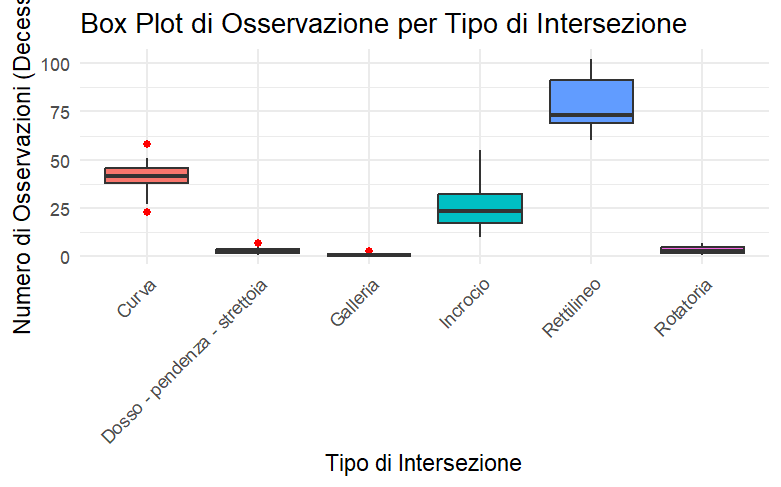
\includegraphics[width=12cm, height=7cm]{Rplot09.png}

\end{figure}
\noindent
Il grafico permette di confrontare la distribuzione  del numero di decessi per ciascun 
tipo di intersezione. Si possono notare differenze nelle mediane, nella variabilità e 
 nella presenza di 
 \footnote{Si dice outlier un dato anomalo, ossia molto distante dagli altri dati. Vengono solitamente rappresentati come punti individuali.}outlier 
 tra le categorie. Ad esempio, i rettilinei potrebbero 
 mostrare una mediana più alta e una maggiore dispersione.

\newpage

\section{Disuguaglianza di Chebyshev}
La \textbf{disuguaglianza di Chebyshev} fornisce un limite inferiore alla proporzione di dati 
che si trovano entro un certo numero ($k$) di deviazioni standard dalla media campionaria ($s$),
indipendentemente dalla forma della distribuzione. La disuguaglianza afferma che 
almeno $1 - 1/k^2$ dei valori si trova nell'intervallo $[\bar{x} - ks, \bar{x} + ks]$, per $k > 1$.

\begin{center}
\begin{lstlisting}[breaklines=true]
# Disuguaglianza di Chebyshev
# media_generale e dev_std_campionaria sono stati calcolati precedentemente
# media_generale = 27.51, dev_std_campionaria = 29.61
# N_validi = sum(!is.na(dati$Osservazione)) # Numero di osservazioni non NA (79)
N_validi <- sum(!is.na(dati$Osservazione))

# Per k = 2 deviazioni standard
k2 <- 2
lim_inf_k2 <- media_generale - k2 * dev_std_campionaria
lim_sup_k2 <- media_generale + k2 * dev_std_campionaria
prop_teorica_k2 <- 1 - 1/k2^2
prop_osservata_k2 <- sum(dati$Osservazione >= lim_inf_k2 & dati$Osservazione <= lim_sup_k2, na.rm = TRUE) / N_validi

cat(paste0("Disuguaglianza di Chebyshev per k = ", k2, ":\n"))
cat(paste0("  Intervallo (media +/- ", k2, " * dev_std): [", round(lim_inf_k2, 2), ", ", round(lim_sup_k2, 2), "]\n"))
cat(paste0("  Proporzione minima teorica di dati nell'intervallo (almeno): ", round(prop_teorica_k2*100, 2), "%\n"))
cat(paste0("  Proporzione osservata di dati nell'intervallo: ", round(prop_osservata_k2*100, 2), "%\n\n"))

# Per k = 3 deviazioni standard
k3 <- 3
lim_inf_k3 <- media_generale - k3 * dev_std_campionaria
lim_sup_k3 <- media_generale + k3 * dev_std_campionaria
prop_teorica_k3 <- 1 - 1/k3^2
prop_osservata_k3 <- sum(dati$Osservazione >= lim_inf_k3 & dati$Osservazione <= lim_sup_k3, na.rm = TRUE) / N_validi

cat(paste0("Disuguaglianza di Chebyshev per k = ", k3, ":\n"))
cat(paste0("  Intervallo (media +/- ", k3, " * dev_std): [", round(lim_inf_k3, 2), ", ", round(lim_sup_k3, 2), "]\n"))
cat(paste0("  Proporzione minima teorica di dati nell'intervallo (almeno): ", round(prop_teorica_k3*100, 2), "%\n"))
cat(paste0("  Proporzione osservata di dati nell'intervallo: ", round(prop_osservata_k3*100, 2), "%\n"))
\end{lstlisting}
\end{center}

\noindent
Output:
\begin{verbatim}
Disuguaglianza di Chebyshev per k = 2:
  Intervallo (media +/- 2 * dev_std): [-31.7, 86.72]
  Proporzione minima teorica di dati nell'intervallo (almeno): 75%
  Proporzione osservata di dati nell'intervallo: 93.59%

Disuguaglianza di Chebyshev per k = 3:
  Intervallo (media +/- 3 * dev_std): [-61.3, 116.33]
  Proporzione minima teorica di dati nell'intervallo (almeno): 88.89%
  Proporzione osservata di dati nell'intervallo: 100.00%
\end{verbatim}
\noindent
Per $k=2$, la disuguaglianza di Chebyshev garantisce che almeno 
il 75\% dei dati si trovi nell'intervallo $[-31.7, 86.72]$. 
Poiché il numero di osservazioni non può essere negativo, l'
intervallo effettivo considerato per i dati è $[1, 86.72]$ 
(essendo 1 il minimo osservato). La proporzione osservata di
 dati in questo intervallo è del 93.59\%, che soddisfa ampiamente 
 il limite teorico.\\\\
Per $k=3$, almeno l'88.89\% dei dati dovrebbe trovarsi nell'
intervallo $[-61.3, 116.33]$ (effettivamente $[1, 102]$ per 
i nostri dati, dato che il massimo è 102). In questo caso, il
 100\% delle osservazioni valide ricade in questo intervallo, 
 confermando la disuguaglianza.


\chapter{Dati Bivariati}
In questa sezione analizzeremo la relazione tra due variabili 
quantitative: l'Anno di riferimento e il Numero Totale di Morti 
annuali per incidenti stradali (limitatamente alla fascia di età 
21-24 anni, conducenti). Useremo i dati aggregati in
 \texttt{morti\_per\_anno}.

\section{Diagramma a dispersione}
Un diagramma a dispersione (scatter plot) mostra la relazione tra due variabili quantitative.

\begin{center}
\begin{lstlisting}[breaklines=true]
# Converti gli anni in numerici per la regressione
if (!is.numeric(morti_per_anno$TIME_PERIOD)) {
  morti_per_anno$TIME_PERIOD_Numeric <- as.numeric(as.character(morti_per_anno$TIME_PERIOD))
} else {
  morti_per_anno$TIME_PERIOD_Numeric <- morti_per_anno$TIME_PERIOD
}

# Crea lo scatter plot
scatter_plot_annuale <- ggplot(morti_per_anno, aes(x = TIME_PERIOD_Numeric, y = Totale_Morti)) +
  geom_point(color = "dodgerblue", size = 3) +
  geom_smooth(method = "lm", se = FALSE, color = "salmon") + # Aggiunge retta di regressione (opzionale qui, ma utile)
  labs(title = "Diagramma a Dispersione: Totale Morti vs. Anno",
       subtitle = "Conducenti 21-24 anni, periodo 2010-2023",
       x = "Anno",
       y = "Numero Totale di Morti") +
  scale_x_continuous(breaks = seq(min(morti_per_anno$TIME_PERIOD_Numeric, na.rm=T),
                                  max(morti_per_anno$TIME_PERIOD_Numeric, na.rm=T), by = 1)) + # Assicura che gli anni siano interi
  theme_minimal()

print(scatter_plot_annuale)
\end{lstlisting}
\end{center}

\begin{figure}[H]
    \centering
    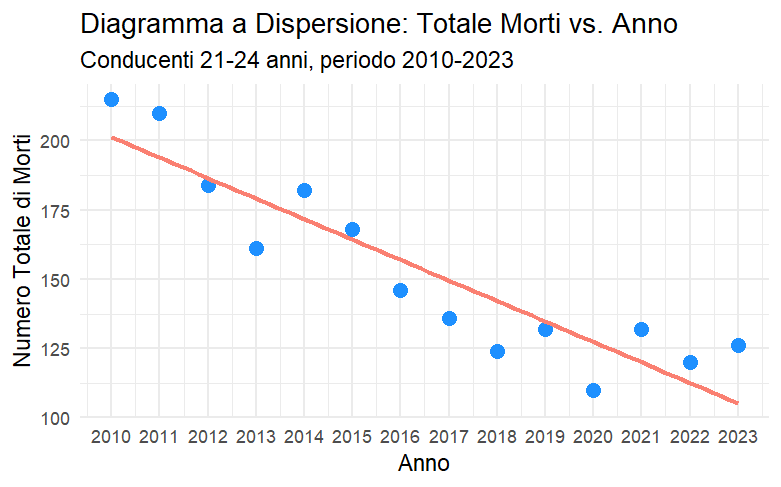
\includegraphics[width=12cm, height=7cm]{Rplot010.png}
\end{figure}

\noindent
Il diagramma a dispersione mostra il numero totale di morti per 
incidenti stradali (nella fascia di età 21-24 anni, conducenti)
per ciascun anno dal 2010 al 2023. Ogni punto blu rappresenta 
un anno. La linea color salmone rappresenta la \textbf{retta di regressione}
lineare, che suggerisce l'andamento generale dei dati nel tempo.
L'area rosa attorno alla retta indica l'intervallo di confidenza 
al 95\% per la stima della media. Visivamente, si osserva una 
tendenza generale alla diminuzione del numero di morti nel corso 
degli anni considerati, sebbene con alcune fluttuazioni.

\section{Coefficiente di correlazione campionario}
Il \textbf{coefficiente di correlazione campionario ($r$)} è una misura normalizzata della forza 
e della direzione della relazione lineare tra due variabili quantitative. Varia tra -1 e +1.
\begin{itemize}
    \item $r = +1$: perfetta correlazione lineare positiva.
    \item $r = -1$: perfetta correlazione lineare negativa.
    \item $r \approx 0$: assenza di correlazione lineare (o relazione lineare molto debole).
    \item Valori vicini a +1 o -1 indicano una forte relazione lineare, mentre valori vicini a 0 indicano una relazione lineare debole o assente.
\end{itemize}

\begin{center}
\begin{lstlisting}[breaklines=true]
# Calcolo del coefficiente di correlazione tra Anno e Totale Morti
correlazione_annuale <- cor(morti_per_anno$TIME_PERIOD_Numeric, morti_per_anno$Totale_Morti, use = "complete.obs", method = "pearson")
print(paste("Coefficiente di correlazione campionario tra Anno e Totale Morti:", round(correlazione_annuale, 4)))
\end{lstlisting}
\end{center}

\noindent
Output:
\begin{verbatim}
"Coefficiente di correlazione campionario tra Anno e Totale Morti: -0.9132"
\end{verbatim}
\noindent
Un coefficiente di correlazione campionario di circa -0.9132 indica una \textbf{forte relazione lineare negativa} tra l'anno e il numero totale di morti. \\\\
\noindent
Ciò conferma in modo più standardizzato l'osservazione precedente: all'avanzare degli anni, si è osservata una marcata tendenza alla diminuzione del numero di decessi per incidenti stradali tra i conducenti di età compresa tra 21 e 24 anni nel periodo 2010-2023.



\end{document}